\chapter{High Level Design}
\label{chp:high_level_design}
\section{Related Work}
\section{Processor Design}
\section{File format}
\section{Memory Latency}
\begin{figure}
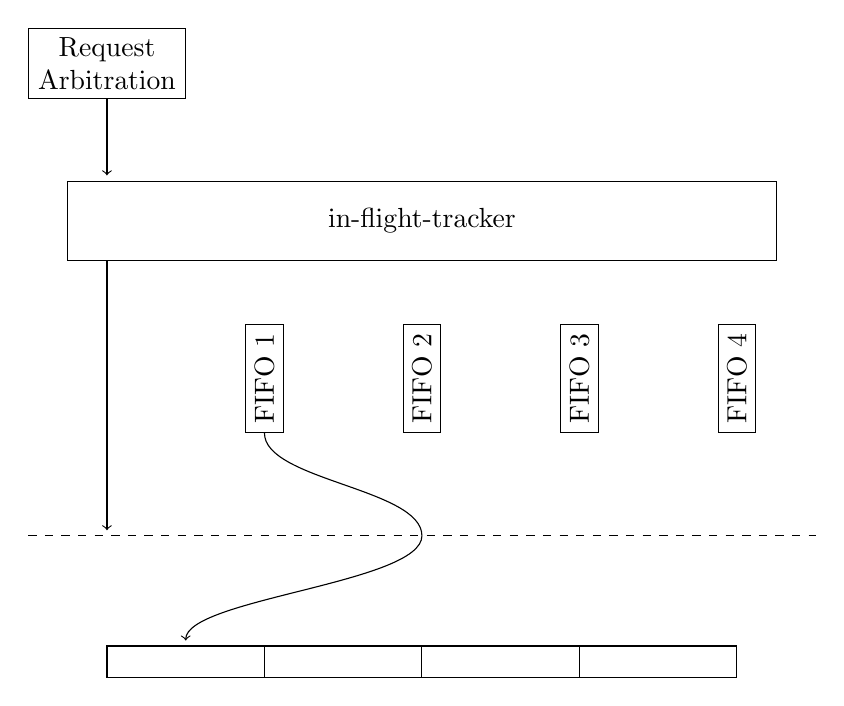
\begin{tikzpicture}[xscale=2,yscale=2]
\node(req) at (0,0) [draw]{\shortstack{Request\\Arbitration}};
\node(tracker) at (2,-1) [draw, minimum width=9cm, minimum height=1cm]{in-flight-tracker};
\node(f1) at (1, -2) [draw,rotate=90]{FIFO 1};
\node(f2) at (2, -2) [draw,rotate=90]{FIFO 2};
\node(f3) at (3, -2) [draw,rotate=90]{FIFO 3};
\node(f4) at (4, -2) [draw,rotate=90]{FIFO 4};
\draw[dashed] (-.5,-3) -- (4.5,-3);
\draw (0,-3.7) -- (4,-3.7) -- (4,-3.9) -- (0,-3.9) -- cycle;
\draw (1,-3.7) -- (1,-3.9);
\draw (2,-3.7) -- (2,-3.9);
\draw (3,-3.7) -- (3,-3.9);

\draw [->,shorten >=2pt] (req) -- (tracker.north -| req);
\draw [->,shorten >=2pt] (tracker.south -| req) -- (0,-3 -| req);
\draw [->,shorten >=2pt] (f1.west) .. controls +(0,-.3) and +(0,.3) .. (2,-3) .. controls +(0,-.3) and +(0,.3) .. (.5,-3.7);

\end{tikzpicture}
\caption{Memory Request Arbitration}
\label{fig:memory_latency}
\end{figure}
Dealing with memory latency is not trivial. The difficulty lies in the fact we are reading 4 streams at different rates. Our platform has a 700 clock cycle external memory latency. We created a general approach with one tweak to achieve high throughput under these conditions.

The hardware consists of 3 parts. First, 4 FIFOs buffer the memory responses of the 4 different streams. Second, an `in-flight-tracker' keeps track of the number of requests to ensure the FIFOs never overflow or have to stall the memory. Third, the request logic determines which (if any) stream should be read from on the current clock cycle.

We use a round robin for request arbitration. We use 3 different signals to determine when to move to the next stream: the tracker information, FIFO saturation and time. First, if the tracker indicates that the limit of in-flight requests has been reached the request arbiter switches to the next stream. Second, if the FIFO corresponding to the to the current stream is half full (indicating that the stream does not need to be read from so often) then the request arbiter switches to the next stream. Third, a timer insures each well get at most 32 requests before the request arbiter switches to the next stream.

\par In practice this still does not achieve good throughput when computing memory bound (difficult to compress) matrices. The problem is that the fzip argument stream (the non-encoded bits or common value index stream) ends up starving and slows down the decoder. To solve this we give priority to this stream by only moving from it when the tracker indicates no more in flight messages can be accepted. This means the timer and the FIFO saturation will not cause the request arbiter to stop reading this stream.
%TODO: explain why
\section{System Design}
\section{Results}
$R^3$, our previous work, achieved up to 13.6 GFLOPS and an average performance of 6 GFLOPS on the non-pattern matrices used by \cite{prelim:bell}. We were able to nearly double this performance to an average of 11 GFLOPS.

\begin{figure*}
\centering
\begin{tikzpicture}[scale=1]

 \ifthenelse{\equal{\blackandwhite}{true}}{
	\tikzstyle{yellowStar}=[draw, diamond, fill=black!65, inner sep =1.5pt];
	\tikzstyle{blueGreenDiamond}=[draw, diamond, fill=black!75, inner sep =1.5pt];
	\tikzstyle{greenSquare}=[draw, rectangle, fill=black!50, inner sep =2.5pt];
	\tikzstyle{blueTriangle}=[draw, regular polygon, regular polygon sides=3, fill=black!35, inner sep =1.5pt];
 }{
	\tikzstyle{yellowStar}=[draw, star, star points=5, fill=yellow, inner sep =1.5pt];
	%\tikzstyle{blueGreenDiamond}=[draw, diamond, fill=green!60!blue, inner sep =1.5pt];
	\tikzstyle{blueGreenDiamond}=[draw, diamond, fill=black, inner sep =1.5pt];
	\tikzstyle{greenSquare}=[draw, rectangle, fill=green, inner sep =2.5pt];
	\tikzstyle{blueTriangle}=[draw, regular polygon, regular polygon sides=3, fill=blue, inner sep =1.5pt];
 }

%\draw [ystep=2.0,gray,very thin, xstep = 14] (0,0) grid (12.9, 6.9);
\draw [->,thick] (0,0) to (14.5, 0);
\draw [->, thick] (0,0) to (0,7);
\foreach \x/\mat/\size in { %
0/dw8192/42K, 1/t2d\_q9/87K, 2/epb1/95K, 3/raefsky1/290K, 4/psmigr\_2/540K, 6/torso2/1M%
}
	\draw (\x cm, 1pt) -- (\x cm, -1pt) node[anchor=east,rotate=90,gray] {\shortstack{\mat (\size)}};
\foreach \x/\mat/\size in { %
5/scircuit/960K, 7/mac\_econ/1.3M, 8/qcd5\_4/1.9M, 9/mc2depi/2.1M, 10/rma10/2.3M, 11/shipsec1/3.6M, 12/dense/4M, 13/cant/4M, 14/consph/6M%
}
	\draw (\x cm, 1pt) -- (\x cm, -1pt) node[anchor=east,rotate=90] {\shortstack{\mat (\size)}};
\foreach \y/\ytext in {0/0,1/5,2/10, 3/15, 4/20, 5/25, 6/30}
	\draw (1pt, \y cm) -- (-1pt, \y cm) node[anchor=east] {$\ytext$};
%\node at (6, -.8) {Size of Matrix (Millions)};
\node at (-1, 3) [rotate=90]{Performance (Gflops)};

%R3 line
\foreach \i/\j/\k/\l in {%
0/0.42000000000000004/1/0.76,  1/0.76/2/0.6599999999999999,  2/0.6599999999999999/3/1.04,  3/1.04/4/0.9800000000000001,  4/0.9800000000000001/5/1.24,  5/1.24/6/1.28,  6/1.28/7/1.1800000000000002,  7/1.1800000000000002/8/2.56,  8/2.56/9/1.24,  9/1.24/10/2.7199999999999998,  10/2.7199999999999998/11/1.58,  11/1.58/12/2.7199999999999998,  12/2.7199999999999998/13/2.54,  13/2.54/14/1.7399999999999998
}{
 \ifthenelse{\equal{\blackandwhite}{true}}{
	\draw [black] (\i,\j) -- (\k,\l);
 }{
	\draw [red] (\i,\j) -- (\k,\l);
 }
}

%hc1 line
\foreach \i/\j/\k/\l in {%
0/0.33999999999999997/1/0.5,  1/0.5/2/0.52,  2/0.52/3/0.78,  3/0.78/4/0.78,  4/0.78/6/0.24
}{
 \ifthenelse{\equal{\blackandwhite}{true}}{
	\draw [black!65] (\i,\j) -- (\k,\l);
 }{
	\draw [brown] (\i,\j) -- (\k,\l);
 }
}

%%tesla line
%\foreach \i/\j/\k/\l in {%
%0/0.1/1/0.18,  1/0.18/2/0.16,  2/0.16/3/0.5599999999999999,  3/0.5599/5/0.6}
%	\draw <3,5>[green!60!blue] (\i,\j) -- (\k,\l);
%newline

%m2090 line
\foreach \i/\j/\k/\l in {%
5/1.2/7/1.2,  7/1.2/8/4.0,  8/4.0/9/4.4,  9/4.4/10/2.2,  10/2.2/11/2.2,  11/2.2/12/4.6,  12/4.6/13/3.4,  13/3.4/14/3.0
}{
 \ifthenelse{\equal{\blackandwhite}{true}}{
	\draw [black!50] (\i,\j) -- (\k,\l);
 }{
	\draw [green] (\i,\j) -- (\k,\l);
 }
}

%intel line
\foreach \i/\j/\k/\l in {%
5/2.4/7/4.6,  7/4.6/8/6.0,  8/6.0/9/4.2,  9/4.2/10/4.8,  10/4.8/11/2.0,  11/2.0/12/2.8,  12/2.8/13/2.4,  13/2.4/14/2.2
}{
 \ifthenelse{\equal{\blackandwhite}{true}}{
	\draw [black!35] (\i,\j) -- (\k,\l);
 }{
	\draw [blue] (\i,\j) -- (\k,\l);
 }
}

\foreach \i/\j/\k/\l in {%
0/0.42000000000000004/1/0.8699999999999999,  1/0.8699999999999999/2/0.95,  2/0.95/3/2.06,  3/2.06/4/2.2800000000000002,  4/2.2800000000000002/5/2.18,  5/2.18/6/2.2199999999999998,  6/2.2199999999999998/7/2.2199999999999998,  7/2.2199999999999998/8/2.68,  8/2.68/9/2.3,  9/2.3/10/2.7800000000000002,  10/2.7800000000000002/11/2.04,  11/2.04/12/2.7,  12/2.7/13/2.66,  13/2.66/14/2.02
}{
 \ifthenelse{\equal{\blackandwhite}{true}}{
	\draw [black!35] (\i,\j) -- (\k,\l);
 }{
	\draw [black] (\i,\j) -- (\k,\l);
 }
}

%\draw [dashed] (.5, -.5) -- (.5, 7) node [fill=white,inner sep=0pt, midway,below, sloped]{\small $(64K)$};

%\draw [dashed] (10.5, -.5) -- (10.5, 7)  node [fill=white,inner sep=0pt, near end,below, sloped]{\small 20MB $(2.5M)$};



%hc1 points
\foreach \i/\x/\y/\f/\q/\u in {%
0/0.083492/0.33999999999999997/1.7/0/-.2,%
1/0.17405/0.5/2.5/0/-.1,%
2/0.190106/0.52/2.6/0/-.2,%
3/0.588552/0.78/3.9/0/-.2,%
4/1.080044/0.78/3.9/0/-.2,%
6/2.066946/0.24/1.2/0/0
}{
 \ifthenelse{\equal{\blackandwhite}{true}}{
	\draw (\i,\y) node[yellowStar]{} node[fill=white,inner sep=0pt, anchor=west,rotate=30,xshift=\q cm + 3pt, yshift=\u cm] {\color{black!65} \scriptsize $\f$};
 }{
	\draw (\i,\y) node[yellowStar]{} node[fill=white,inner sep=0pt, anchor=west,rotate=30,xshift=\q cm + 3pt, yshift=\u cm] {\color{brown} \scriptsize $\f$};
 }
}	

%intel points
\foreach \i/\x/\y/\f/\q/\u in {%
5/1.917872/2.4/12/0/0,%
7/2.546778/4.6/23/0/0,%
8/3.833856/6.0/30/0/0,%
9/4.20045/4.2/21/0/-.2,%
10/4.658184/4.8/24/0/0,%
11/7.136352/2.0/10/0/0,%
12/8.0/2.8/14/0/.2,%
13/8.014766/2.4/12/0/-.2,%
14/12.02096/2.2/11/0/0
}{
 \ifthenelse{\equal{\blackandwhite}{true}}{
	\draw (\i cm,\y cm) node[blueTriangle]{} node[fill=white,inner sep=0pt, anchor=west,rotate=30,xshift=\q cm + 3pt, yshift=\u cm]{\color{black!50} \scriptsize $\f$};
 }{
	\draw (\i cm,\y cm) node[blueTriangle]{} node[fill=white,inner sep=0pt, anchor=west,rotate=30,xshift=\q cm + 3pt, yshift=\u cm]{\color{blue} \scriptsize $\f$};
 }
}

%M2090 points
\foreach \i/\x/\y/\f/\q/\u in {%
5/1.917872/1.2/6/0/-.3,%
7/2.546778/1.2/6/0/.3,%
8/3.833856/4.0/20/0/0,%
9/4.20045/4.4/22/0/0,%
10/4.658184/2.2/11/0/0,%
11/7.136352/2.2/11/0/.1,%
12/8.0/4.6/23/0/0,%
13/8.014766/3.4/17/0/0,%
14/12.02096/3.0/15/0/0
}{
 \ifthenelse{\equal{\blackandwhite}{true}}{
	\draw (\i,\y) node[greenSquare]{} node[fill=white,inner sep=0pt, anchor=west,rotate=30,xshift=\q cm + 3pt, yshift=\u cm]{\color{black!35} \scriptsize $\f$};
 }{
	\draw (\i,\y) node[greenSquare]{} node[fill=white,inner sep=0pt, anchor=west,rotate=30,xshift=\q cm + 3pt, yshift=\u cm]{\color{green!100} \scriptsize $\f$};
 }
}

%R3 points
\foreach \i/\x/\y/\f/\q/\u in {%
0/0.083492/0.42000000000000004/2.1/0/0,%
1/0.17405/0.76/3.8/0/0,%
2/0.190106/0.6599999999999999/3.3/0/0,%
3/0.588552/1.04/5.2/0/0,%
4/1.080044/0.9800000000000001/4.9/0/0,%
5/1.917872/1.24/6.2/0/0,%
6/2.066946/1.28/6.4/0/0,%
7/2.546778/1.1800000000000002/5.9/0/0,%
8/3.833856/2.56/12.8/0/0,%
9/4.20045/1.24/6.2/0/0,%
10/4.658184/2.7199999999999998/13.6/0/0,%
11/7.136352/1.58/7.9/0/0,%
12/8.0/2.7199999999999998/13.6/0/0,%
13/8.014766/2.54/12.7/0/0,%
14/12.02096/1.7399999999999998/8.7/0/0
}{
 \ifthenelse{\equal{\blackandwhite}{true}}{
	\draw (\i,\y) [fill=black]circle(3pt) node(r\i)[fill=white,inner sep=0pt, anchor=west,rotate=30,xshift=\q cm + 3pt, yshift=\u cm]{\color{black} \scriptsize $\f$}; 
 }{
	\draw (\i,\y) [fill=red]circle(3pt) node(r\i)[fill=white,inner sep=0pt, anchor=west,rotate=30,xshift=\q cm + 3pt, yshift=\u cm]{\color{red} \scriptsize $\f$};
 }
}
%new points
\foreach \i/\x/\y/\f/\q/\u in {%
0/0.083492/0.42000000000000004/2.1/0/0,%
1/0.17405/0.8699999999999999/4.35/0/0,%
2/0.190106/0.95/4.75/0/0,%
3/0.588552/2.06/10.3/0/0,%
4/1.080044/2.2800000000000002/11.4/0/0,%
5/1.917872/2.18/10.9/0/0,%
6/2.066946/2.2199999999999998/11.1/0/0,%
7/2.546778/2.2199999999999998/11.1/0/0,%
8/3.833856/2.68/13.4/0/0,%
9/4.20045/2.3/11.5/0/0,%
10/4.658184/2.7800000000000002/13.9/0/0,%
11/7.136352/2.04/10.2/0/0,%
12/8.0/2.7/13.5/0/0,%
13/8.014766/2.66/13.3/0/0,%
14/12.02096/2.02/10.1/0/0
}{
 \ifthenelse{\equal{\blackandwhite}{true}}{
	\draw (\i,\y) node[greenSquare]{} node[fill=white,inner sep=0pt, anchor=west,rotate=30,xshift=\q cm + 3pt, yshift=\u cm]{\color{black!35} \scriptsize $\f$};
 }{
	\draw (\i,\y) node[blueGreenDiamond]{} node[fill=white,inner sep=0pt, anchor=west,rotate=30,xshift=\q cm + 3pt, yshift=\u cm]{\color{black!100} \scriptsize $\f$};
 }
}

\draw (4,5.5) node (key)[rectangle,minimum width=4cm, minimum height=2.7cm]{};
 \ifthenelse{\equal{\blackandwhite}{true}}{
	\node at (key) [rectangle,anchor=west, xshift=-2cm, yshift=1cm]{\tikz{\draw (0,1pt) [fill=black]circle (2.5pt);} $R^3$};
 }{
	\node at (key) [rectangle,anchor=west, xshift=-2cm, yshift=1cm]{\tikz{\draw (0,1pt) [fill=red]circle (2.5pt);} $R^3$};
 }
\node at (key) [rectangle,anchor=west, xshift=-2cm, yshift=1.7cm]{\shortstack{\tikz{\draw (0,1pt) node[blueGreenDiamond]{};} New Design}};
\node at (key) [rectangle,anchor=west, xshift=-2cm, yshift=.3cm]{\shortstack{\tikz{\draw (0,1pt) node[yellowStar]{};} \cite{prelim:nagar1} }};
%\node <3,5>at (key) [rectangle,anchor=west, xshift=-2cm, yshift=0cm]{\tikz{\draw (0,1pt) node[blueGreenDiamond]{};} Nvidia Tesla S1070};
\node at (key) [rectangle,anchor=west, xshift=-2cm, yshift=-.5cm]{\shortstack{\tikz{\draw (0,1pt) node[greenSquare]{};} Nvidia Tesla \\M2090}};
\node at (key) [rectangle,anchor=west, xshift=-2cm, yshift=-1.5cm]{\shortstack{\tikz{\draw (0,1pt) node[blueTriangle]{};} Intel E5-2690 \\(2 CPUs)}};

\end{tikzpicture}
\caption[SpMV performance on our newest design]{$nnz$ vs Performance on each platform. As seen we only get a small increase in performance compared to $R^3$ when $R^3$ already achieves a relatively high performance.}
\label{fig:newResults}
\end{figure*}

Some trends do appear. Like in $R^3$ the new design does not achieve good performance on the 3 smallest matrices. This is due to the memory latency of the platform. In fact, the smallest matrix (dw8192) is so small that all of the read requests occur before the first value is multiplied.

Another trend is that the more compressible matrices achieve the best performance. The 3 pattern matrices (qcd5\_4, rma10, and dense) achieve the best performance.

In terms of area about half of the Xilinx Virtex-6 LX760 FPGA is utilized. The uses 255K out of 948K registers, 224K out of 474K LUTs, 515 out of 720 RAM blocks, 112 out of 864 DSPs (multiplier blocks).
